\documentclass[12pt,english,brazil,a4paper,utf8,oneside]{utfpr-tcc}

% Este comando não é necessário: utilizei apenas para deixar o latex2rtf
% feliz (e descobrir a codificação do texto).
\usepackage[utf8]{inputenc}

% Suporte a figuras e subfiguras
\usepackage{graphics}
\usepackage{subfigure}

% Suporte a tabelas (principalmente do cronograma)
\usepackage{tabularx}
\usepackage{multirow}
\usepackage{array}
\usepackage{tabularx}
\usepackage{colortbl}
\usepackage{hhline}
\usepackage{xcolor}

% Elementos geralmente utilizados na tabela do cronograma
\newcommand{\fullcell}{\multicolumn{1}{>{\columncolor[gray]{0.5}}c}{}}
\newcommand{\fullcellline}{\multicolumn{1}{>{\columncolor[gray]{0.5}}c|}{}}
\newcommand{\mc}[3]{\multicolumn{#1}{#2}{#3}}
\newcommand{\y}{\rule{8pt}{4pt}}
\newcommand{\n}{\hspace*{8pt}} 

% Define o caminho das figuras
\graphicspath{{images/}}

% Dados do curso que não precisam de alteração
\university{Universidade Tecnológica Federal do Paraná}
\universityen{Federal University of Technology -- Paraná}
\universityunit{Departamento Acadêmico de Computação}
\address{Campo Mourão}
\addressen{Campo Mourão, PR, Brazil}
\documenttype{Monografia}
\documenttypeen{Monograph}
\degreetype{Graduação}


%%%%%%%%%%%%%%%%%%%%%%%%%%%%%%%%%%%%%%%%%%%%%%%%%%%%%%%%%%%%%%%%%%%%%%%%%%%%%
% Alterar daqui para baixo
%%%%%%%%%%%%%%%%%%%%%%%%%%%%%%%%%%%%%%%%%%%%%%%%%%%%%%%%%%%%%%%%%%%%%%%%%%%%%

% Dados do curso. Caso seja BCC:
\program{Curso de Bacharelado em Ciência da Computação}
\programen{Undergradute Program in Computer Science}
\degree{Bacharel}
\degreearea{Ciência da Computação}
% Caso seja TSI:
% \program{Curso Superior de Tecnologia em Sistemas para Internet}
% \programen{Undergradute Program in Tecnology for Internet Systems}
% \degree{Tecnólogo}
% \degreearea{Tecnologia em Sistemas para Internet}


% Dados da disciplina. Escolha uma das opções e a descomente:
% TCC1:
\goal{Proposta de Trabalho de Conclusão de Curso de Graduação}
\course{Trabalho de Conclusão de Curso 1}
% TCC2:
% \goal{Trabalho de Conclusão de Curso de graduação}
% \course{Trabalho de Conclusão de Curso 2}


% Dados do TCC (precisa alterar)
\author{}  % Seu nome
\title{} % Título do trabalho
\titleen{} % Título traduzido para inglês
\advisor{} % Nome do orientador. Lembre-se de prefixar com "Prof. Dr.", "Profª. Drª.", "Prof. Me." ou "Profª. Me."}
% \coadvisor{} % Nome do coorientador, caso exista. Caso não exista, comente a linha.
\depositshortdate{2016} % Ano em que depositou este documento

% Dados da ficha catalografica. Ela é opcional, mas é uma boa ideia inserí-la. Exemplos para geração (http://fichacatalografica.sibi.ufrj.br/)
\fichacatautor{}  % Nome conforme citado (ou seja, no formato "Sobrenome, Nome").
\fichacatbib{Biblioteca da UTFPR de Campo Mourão} % Não alterar
\fichacatpum{M488} % Código Cutter-Sanborn. Use a primeira letra do sobrenome seguido do número conforme as primeiras letras do sobrenome e a tabela http://www.amormino.com.br/cutter-sanborn/cutter1.html
\fichacatpalcha{} % Assuntos do trabalho. Cada item deve ser enumerado e separado por ponto: 1. xxx. 2. yyy. 3. zzz.
\fichacatpdois{} % Deixar em branco


\begin{document}
	
\frontmatter
\maketitle

\begin{resumo}
% TODO: se possível, escreva um resumo estruturado. Para TCC 1, o resumo estruturado teria os seguintes elementos:
% \textbf{Contexto:} \\
% \textbf{Objetivo:} \\
% \textbf{Método:} \\
% \textbf{Resultados esperados:} 
% ou, para TCC 2:
% \textbf{Contexto:} \\
% \textbf{Objetivo:} \\
% \textbf{Método:} \\
% \textbf{Resultados:} \\
% \textbf{Conclusões:}

% Palavras-chaves, separadas por ponto (tente não definir mais do que cinco)
\palavraschaves{}
\end{resumo}



% Caso seja TCC 2, precisa traduzir o resumo e as palavras-chaves para inglês:
% \begin{abstract}
% \textbf{Context:}
% \textbf{Objective:}
% \textbf{Method:}
% \textbf{Results:}
% \textbf{Conclusions:}

% Palavras-chaves em inglês, separadas por ponto.
% \keywords{}
% \end{abstract}



% Listas (opcionais, mas recomenda-se a partir de 5 elementos)
\listoffigures
\listoftables

% Sumário
\tableofcontents

\mainmatter
% TODO: incluir arquivos latex com os capítulos
\section{Introdução}

Não é novidade que o termo \textit{`microservices'} injetou grande entusiasmo no mundo da computação. Determinada circunstância verifica-se nos diversos \textit{cases} de sucesso como o são o Netflix e Soundcloud CITE. Este advento, como qualquer novidade, carece de ponderadas análises para solidificar-se e frutificar em meio ao ecossistema já existente.

\subsection{O fenômeno}

O fenômeno que se vê deve-se ao recente impulso que as \textit{start-up's} trouxeram ao mundo, explorando os métodos ágeis de desenvolvimento unido a cultura DevOps. Tão logo lastreou-se na realidade a oferta, necessariamente, lastreara-se a demanda CITE: Em resposta a volatibilidade e efervescência dos requisitos do sistema e ao efeito \textit{jitter} FOOTNOTE que o sistema poderá sofrer no que se refere a flutuação da vazão que a aplicação deverá suportar em termos de número de usuários do \textit{software} que se desejar produzir, cria-se um leque de tecnologias, como o é também a computação em nuvem, cujo propósito intende atendê-los.

Aplicações desenvolvidas sob o modelo de \textit{start-up's} e/ou com a forma de métodos ágeis tende a ser planejado para pequenas quantidades de usuários, de modo que um dos grandes desafios destas empresas é fazer com que sua tecnologia não se degrade com o tempo e consiga acompanhar o crescimento da empresa.

Conforme pode-se visualizar na Figura 2 REF, até a década de 80 construía-se \textit{software} altamente acoplados, de modo que nenhum de seus componentes poderia existir \textit{per se}.

\begin{figure}
\centering
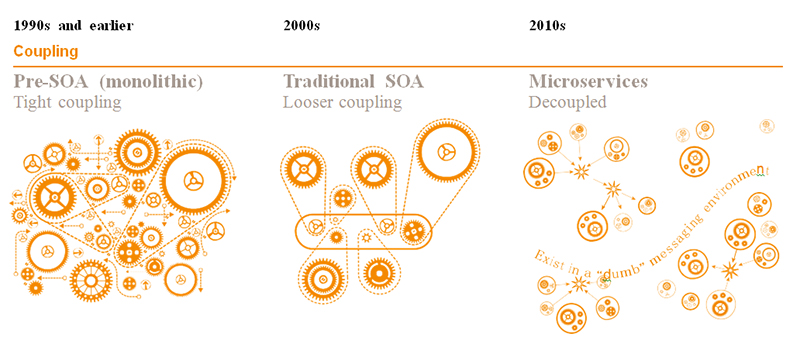
\includegraphics[width=14cm]{feature02-figure02}
\caption{Evolução do desenvolvimento}
\end{figure}

À medida em que crescem o número de usuários de uma aplicação, cresce também a complexidade de atender satisfatoriamente todos os usuários. Neste ponto há a necessidade de escalar aplicações. A Figura 1 REF mostra as formas pelas quais é possível escalar uma aplicação.

\begin{figure}
\centering
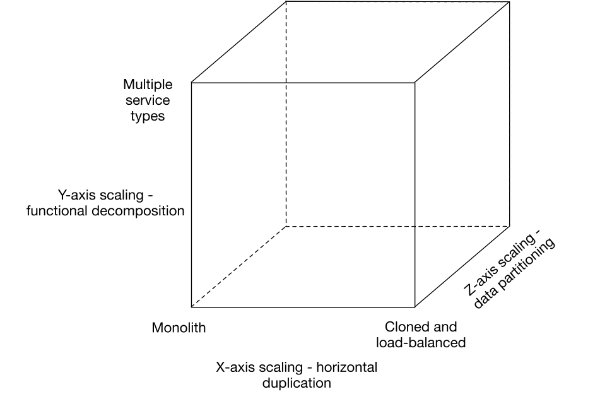
\includegraphics[width=14cm]{scale}
\caption{Escalagem de uma aplicação}
\end{figure}

Tês são os eixos de escala de uma aplicação conforme demonstra CITE: É possível clonar a aplicação, o que implica em orquestrar o \textit{gateway} das requisições; Possível particionar os dados, o dito \textit{sharding}, o que implica em orquestrar o acesso aos dados; E ainda, é possível, cindir uma aplicação em micro-serviços, o que implica em orquestrar os serviços. Uma aplicação centrada na origem, isto é, sem qualquer forma de escalagem, é uma aplicação monolítica.

Sumariamente, constata-se um movimento que contribui para que o desenvolvimento inicie-se em tamanho reduzido e depois sofra, incrementalmente, a necessidade de expandí-lo e servir mais usuários. Há, portanto, um movimento que induz aos desenvolvedores de \textit{software} cogitar a hipótese dos micro-serviços.

\subsection{Os micro-serviços}

Sob este olhar, cumpre definir o termo: Micro-serviços é uma arquitetura de \textit{software} cuja finalidade é reduzir o acoplamento entre os diversos módulos de uma aplicação com o propósito de facilitar sua escalagem. Ao seu oposto dá-se o nome de aplicação monolítica cujos diversos módulos residem na mesma aplicação e comunicam-se diretamente por meio chamadas de métodos. Nesta, nenhuma funcionalidade do sistema existe e opera por si só. Como efeitos colaterais da adoção da arquitetura de micro-serviços adiquirem-se benefícios e malefícios a depender do aspecto sobre o qual se olha.

Deste modo, uma aplicação desenvolvida sob esta arquitetura identifica-se por possuir vários \textit{softwares} cada qual com uma única e bem específica responsabilidade. A métrica para cindir um módulo deve sempre ser a sincera análise do \textit{trade-off} que há em cindir a aplicação ou mantê-la aglutinada. Em linhas gerais, vale sempre a necessidade de cada aplicação. Isto é: Uma vez que uma parte da aplicação precise ser escalada ou sofra constante modificação, pensa-se em decompô-la. Do contrário, mantenha-se a aplicação aglutinada.

Ao adotar esta arquitetura os desenvolvedores vêem-se em face a maior facilidade ao realizar testes unitários no sentido de que poucos serão os arquivos a serem analisados e pouco complexa será a aplicação, uma vez que parte do todo. De outra banda, dificuldades nos testes de integração, uma vez que todo o cenário, que complexo de ser implementado, precisa ser estar em atividade para que os testes sejam realizados; Facilidade na manutenção e dificuldade na implantação são faces da mesma moeda no que tange a arquitetura de micro-serviços.

Naturalmente estes \textit{trade-off's} são contornados com algumas ferramentas que propõe fazê-lo. Para a facilitar a implantação de um sistema distribuído, utilizam-se contêineres, que respondem por isolar uma aplicação em seu ambiente ideal de um determinado micro-serviço que compõe a aplicação; Para orquestrar a escalagem; Para testar em produção, chaos monkey. CITE.

Embora a literatura aponte que ao assumir uma arquitetura de micro-serviços, adiciona-se 70\% de sobrecarga ao sistema devido ao \textit{overhead}, existem classes de aplicações, como apontado, que cumprem melhor seu papel sob a égide dos micro-serviços. De modo que, sem dúvida, um grande passo na vida da empresa é decidir por adotar ou não micro-serviços. Decidir migrar ou não sua aplicação para a nuvem também deve ser uma escolha delicada que a empresa terá que fazer.

\subsection{Seu desenvolvimento}

É bem verdade que o desenvolvimento de um \textit{software} deve seguir a engenharia lógica do mapeamento do mundo real para o computacional. Há, primeiro, a necessidade de capturar o fluxo de trabalho (\textit{workflow}) que se deseja automatizar para só então escolher a arquitetura de \textit{software} que mais se adequa ao \textit{workflow} que traduzirá a aplicação. Desta feita, os desenvolvedores poderão optar por utilizar ou não micro-serviços. É só após esta qualidade de decisões que poderão ser aplicados padrões de micro-serviços e padrões de projeto.

Quando uma aplicação é feita ``sob medida'' para públicos grandes, não existem grandes surpresas, isto é, os desenvolvedores já possuem clareza de que a aplicação deverá ser elástica, tolerante a falhas e facilmente manutenível. Tão logo, a opção por um cenário composto por micro-serviços pode ser bem clara. Tão logo, a terceirização da hospedagem na nuvem poderá ser uma opção. Sobretudo, deixar de incorrer na necessidade de manutenir esse aspecto ``em produção'', faz com que o sistema seja erigido já sob o aparato articulatório que a necessidade de escalagem demanda.

Quando uma aplicação é feita para públicos pequenos, não raras vezes, não há engenharia que introduza resiliência ao \textit{software}, de modo que se o sucesso bate à porta da empresa, não raras vezes o custo de atender ao sucesso exorbita o planejamento.

É imperioso que uma aplicação possua elasticidade de código sem esfacelar-se perante novas funcionalidades. Não há quem não saiba que o custo de manutenção de um \textit{software} cresce à medida em que o mesmo ganha volume, especialmente quando não houver fidelidade à regra de negócio que a aplicação mapeia. É por isso que recomenda-se que as aplicações que inicialmente planejem-se para servir pequenos públicos, planejem-se igualmente para escalar sua aplicação no futuro. Quanto mais postergado for o planejamento, tanto mais custosa será a manutenção.

Seja ela feita ``sob medida'' para grandes públicos, seja ela feita ``sob medida'' para pequenos públicos, o fato porém é que ocasionalmente a aplicação precisará migrar para uma arquitetura de micro-serviços.

Neste cenário, duas são as abordagens a se considerar no que tange o desenvolvimento de aplicações orientada a micro-serviços: O desenvolvimento gradual de uma aplicação já orientada a micro-serviços e a transição gradual de um sistema para esta arquitetura. Decerto cada abordagem possui seus busílis, os quais serão esmiuçados nas linhas que seguem.

\subsection{Desenvolvimento gradual}

Quando uma aplicação crescer desde pequena já orientada a micro-serviços é evidente que a complexidade de escalá-la será menor, uma vez que não serão necessárias quaisquer adaptações ou, pior, mudanças drásticas ``em produção''.

Ao fim das contas é admissível um cenário em que diversas tecnologias, linguagens e meios de comunicação sejam adotados a depender da necessidade do produto, da regra de negócio da aplicação, da demanda dos usuários e da facilidade com a qual cada funcionalidade do sistema é implementada em determinadas linguagens, ferramentas ou meios de comunicação. A figura REF demonstra.

\begin{figure}
\centering
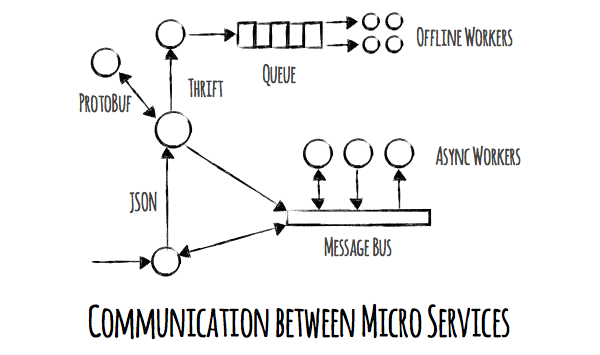
\includegraphics[width=14cm]{micro-service-architecture-comms}
\caption{Cenário de comunicação poliglota}
\end{figure}

É claro que adquirir a possibilidade de um sistema heterogêneo é interessante, contudo cabe salientar que não deve-se adicionar grau de heterogeneidade mais elevado do que a empresa possa gerir.

A construção de um sistema orientado a arquitetura de micro-serviços assemelha-se à reconstrução de um sistema. Alguns passos devem ser seguidos em ambas abordagens exceto por seguras exceções.

\subsection{Transição gradual}

Quando uma aplicação precisar sofrer a transição para a arquitetura de micro-serviços e já estiver servindo seus usuários, muitos cuidados deverão ser tomados para que o serviço aos usuários não seja prejudicado, tampouco seus dados.

De início, é importante compreender que desajustes impostos ao sistema produzem desajustes em cascata para todos os degraus inferiores. Este fenômeno, amplamente conhecido por qualquer um que se atreva a projetar um sistema, aplica-se tanto ao desenvolvimento quanto aos protocolos e planejamentos.

Bem, se assim é verdade, decompor um sistema monolítico em micro-serviços pode ser uma tarefa laborosa se houverem imperfeições arquiteturais no sistema, de modo que é necessário buscar corrigir tais imperfeições de maneira a minimizar a complexidade que sabidamente será adicionada ao sistema ao cindí-lo em microserviços.

Assim sendo, como todo ponto de partida de um \textit{software} é o \textit{workflow} que ele implementa, esta é a primeira etapa da transição gradual: Revisitar o \textit{workflow}, isto é, a regra do negócio; Se necessário, aplicar padrões. Em seguida, é preciso revisitar a arquitetura do \textit{software} fazendo-o responder aos impulsos do \textit{workflow} que se pretenda automatizar.

Já neste ponto faz-se necessária a firme compreensão dos micro-serviços que comporá o sistema. Existem estratégias para decidir como cindir uma aplicação.

É ainda importante que o projeto do \textit{software} seja revisitado, com o auxílio de seu diagrama de classes, buscando desacoplar componentes. Se necessário aplicar padrões de projeto.

Estando o sistema entregue, isto é, ``em produção'', fará-se necessário o desenvolvimento dos micro-serviços a orbitarem o monolítico adjunto de uma camada de abstração entre ele e o monolítico, comumente chamada como \textit{glue code}. , deve-se erguer duas fachadas que dêem ao usuário do sistema a sensação de que o sistema não está em obras. A figura REF materializa esta ideia.

\begin{figure}
\centering
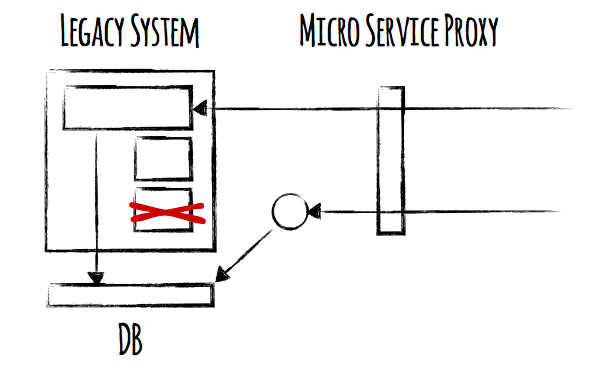
\includegraphics[width=14cm]{micro-service-architecture-proxy}
\caption{Fachada de abstração entre os serviços}
\end{figure}

Se o sistema apresentar arquitetura próxima ao MVC, a primeira cisão a ser feita pode ser justamente nestes três componentes, e entre cada um deles, uma fachada de interface. A primeira, para que o usuário mantenha utilizando a interface antiga. Esta fachada desempenha a função de selecionar qual ambiente processará as requisições do usuário, ou seja, se o sistema monolítico -- que ainda estará em fase de declínio -- ou se o micro-serviço. A segunda fachada abstrairá a persistência, fazendo com que tanto o monolítico quanto os micro-serviços continuem a persistir na mesma e antiga base de dados.

Para o ponto de contato entre as classes de micro-serviços distintos, pode ser adicionado um representante da classe do micro-serviço vizinho, possuinte dos mesmos métodos que será responsável por enviar as solicitações para um \textit{buffer} compartilhado. Utilizar esta estratégia permite que o código não precise ser reescrito nem modificado, apenas que seja criada uma abstração entre o ponto de contato, além de tornar a escalabilidade do sistema natural.

Naturalmente uma questão a se pensar é a comunicação entre os micro-serviços. Algumas ferramentas encarregam-se de abstrair os detalhes da comunicação por meio de injeção de dependência. Um serviço de filas (ou qualquer meio de comunicação indireta) conjugada a um \textit{marshalling} para JSON (ou qualquer outra representação externa de dados) deverá ser utilizada para admitir a heterogeneidade do sistema.

Seja na construção de um novo produto, ou na reconstrução de um produto já existente, o processo descrito precisa ser seguido. Muitas vezes esse processo se dá de maneira automática, contudo é importante que se seja de maneira consciente.

\subsection{Padrões}

Muitas são as formas de se compor um sistema dado que diversos são os problemas a serem solucionados. Chris REF reuniu uma série de problemas e soluções adotadas para eles em seu livro. Cabe consultá-lo quando na necessidade de desenvolver um sistema orientado a micro-serviços.

\begin{figure}
\centering
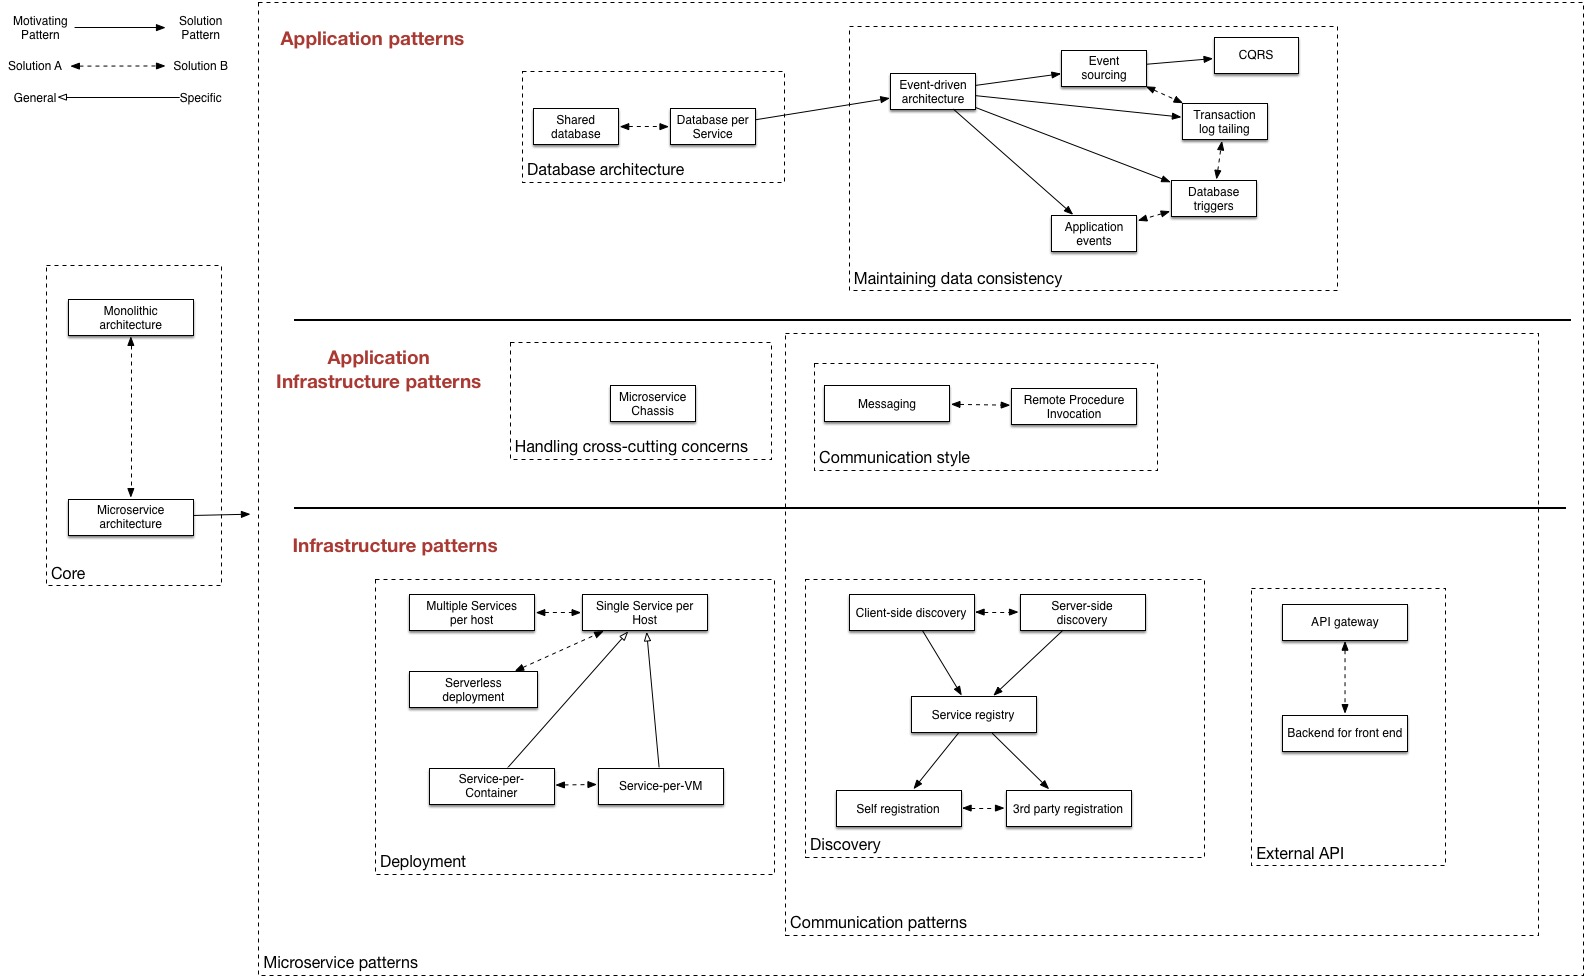
\includegraphics[width=14cm]{MicroservicesPatternLanguage}
\caption{Padrões de micro-serviços}
\end{figure}
% \include{referencial-teorico}
% \include{proposta}
% \include{resultados-preliminares}

\bibliographystyle{abntex2-alf}
\bibliography{main} % geração automática das referências a partir do arquivo main.bib

\backmatter
\end{document}
